\section{Quiz}

This remainder of this homework is a series of multiple choice questions related to the word2vec algorithm.

{\bf How to submit:}  Even though these are not coding questions, you will submit your response to
each question in the |src-quiz/submission.py| file.  This file will act as
your 'bubble sheet' for multiple choice questions in this course.  A sample response
might look like this:

\begin{center}
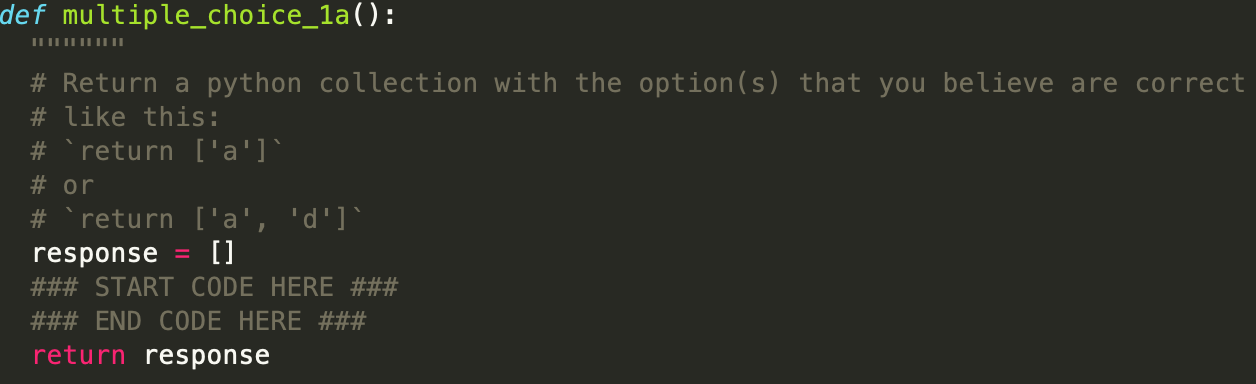
\includegraphics[width=1\textwidth]{sample_question_empty.png}
\end{center}

If you believe that |a| and |b| are the correct responses to this question, you
will type |response = [`a', `b']| between the indicated lines like this:

\begin{center}
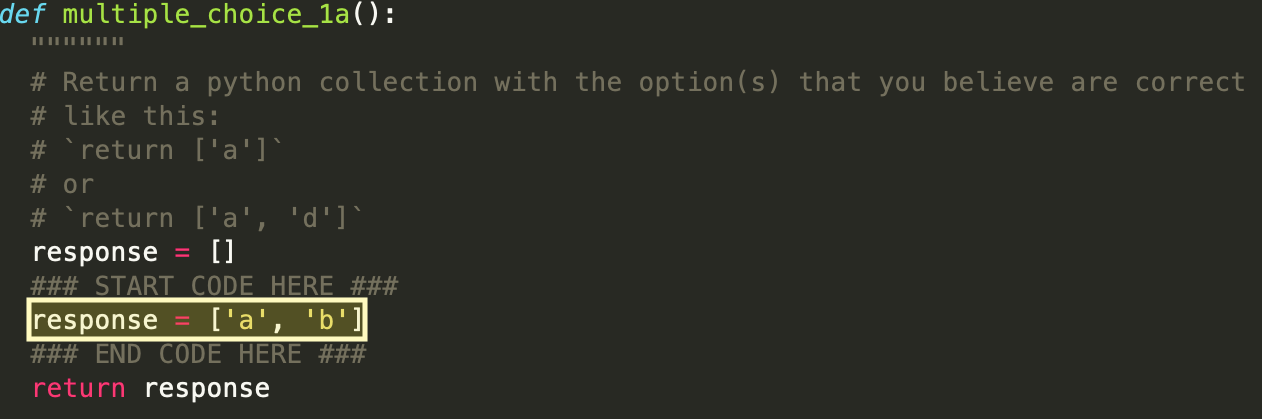
\includegraphics[width=1\textwidth]{sample_question_complete.png}
\end{center}

{\bf How to verify your submission:}
You can run the student version of the autograder locally like all coding
problem sets.  In the case of this problem set, the helper tests will verify
that your responses are within the set of possible choices for each question
(e.g. the helper functions will flag if you forget to answer a question of if
you respond with |[`a', `d']| when the choices are |[`a', `b', `c']|.)  See the
front pages of this assignment for instructions to run the autograder.
\clearpage

\begin{enumerate}[1.]
\item \points{quiz1}
Choose all the equations that represent the differential of a sigmoid (When choosing the right option(s) consider the given input x to be a scalar instead of a vector).
\begin{enumerate}[(a)]
\item \begin{equation*}\frac{\partial \sigma(x)}{\partial x} = {\sigma(x) \cdot (1-\sigma(x))}\end{equation*}
\item \begin{equation*}\frac{\partial \sigma(x)}{\partial x} = 1 - {\sigma(x) \cdot (1-\sigma(x))}\end{equation*}
\item \begin{equation*}\frac{\partial \sigma(x)}{\partial x} = \frac{e^{-x}}{(1+e^{-x})^2}\end{equation*}
\item \begin{equation*}\frac{\partial \sigma(x)}{\partial x} = \frac{ (1-e^{-x})}{(1+e^{-x})^2}\end{equation*}
\end{enumerate}

% ### START CODE HERE ###
% ### END CODE HERE ###

\item \points{quiz2}
What is the shape of the matrices U and V where (please refer to reading material from the handout):

$U$ is the outside vector matrix

$V$ is center vector matrix

|num_tokens|: Number of unique words in the dataset

|embed_size|: size of the word vector(word2vec size)

\begin{enumerate}[(a)]
\item $U$ : (|embed_size| $\times$ 1); $V$ : (|embed_size| $\times$ |num_tokens|)
\item $U$ : (|num_tokens| $\times$ |num_tokens|) ; $V$ : (|embed_size| $\times$ 1)
\item $U$ : (|embed_size| $\times$ |num_tokens|) ; $V$ : (|embed_size| $\times$ |num_tokens|) 
\item $U$ : (|embed_size| $\times$ 1) ; $V$ : (|embed_size| $\times$ 1) 
\end{enumerate}

% ### START CODE HERE ###
% ### END CODE HERE ###

\item \points{quiz3}
What is the shape of the gradient $\frac{\partial J_\text{naive-softmax}}{\partial V_c}$ matrix/vector where:
\begin{equation*} J_{\text{naive-softmax}}(\bm v_c, o, \bm U) = - \bm u_{o}^\top \bm v_c + \log \bigg( \sum_{w' \in \text{Vocab}} \exp(\bm u_{w'}^\top \bm v_c) \bigg) \end{equation*}

\begin{equation*} {\partial J \over \partial \bm v_c} = \bm U(\hat{\bm y} - \bm y)\end{equation*}

$U$ is the outside vector matrix

$\hat{y}$ is the predicted output

$y$ is the actual output

|num_tokens|: Number of unique words in the dataset

|embed_size|: size of the word vector(word2vec size)

\begin{enumerate}[(a)]
\item |num_tokens| $\times$ 1
\item |embed_size| $\times$ 1
\item |embed_size| $\times$ |num_tokens|
\end{enumerate}

% ### START CODE HERE ###
% ### END CODE HERE ###

\item \points{quiz4}
What is the shape of the gradient $\frac{\partial J_\text{naive-softmax}}{\partial U}$ (will be referred to $\frac{\partial J}{\partial U}$ for simplicity) matrix/vector where:

\begin{equation*} J_{\text{naive-softmax}}(\bm v_c, o, \bm U) = - \bm u_{o}^\top \bm v_c + \log \bigg( \sum_{w' \in \text{Vocab}} \exp(\bm u_{w'}^\top \bm v_c) \bigg) \end{equation*}

\begin{equation*} {\partial J \over \partial \bm U } = {\bm v_c} (\hat{\bm y} - \bm y)^\top \end{equation*}

$V_c$ is the center vector

$\hat{y}$ is the predicted output

$y$ is the actual output

|num_tokens|: Number of unique words in the dataset

|embed_size|: size of the word vector(word2vec size)

\begin{enumerate}[(a)]
\item |num_tokens| $\times$ 1
\item |embed_size| $\times$ 1
\item |embed_size| $\times$ |num_tokens|
\end{enumerate}

% ### START CODE HERE ###
% ### END CODE HERE ###

\item \points{quiz5}
Which of the below equations represents a general form of SGD where $g(x)$ is the gradient of loss function and $\eta$ is the learning rate:

\begin{enumerate}[(a)]
\item \begin{equation*}x = {x - eta \cdot g(x)}\end{equation*}
\item \begin{equation*}x = {x - eta \cdot \frac{\partial g(x)}{\partial x}}\end{equation*}
\item \begin{equation*}x = {x - \frac{eta}{g(x)}}\end{equation*}
\item \begin{equation*}x = {x - eta \cdot {\frac{\partial x}{\partial g(x)}}}\end{equation*}
\end{enumerate}

% ### START CODE HERE ###
% ### END CODE HERE ###

\item \points{quiz6}
Negative sampling was briefly introduced the Lecture 2 video Word2Vec: Model Variants. \href{https://stackoverflow.com/questions/27860652/word2vec-negative-sampling-in-layman-term#answer-27864657}{Here} and \href{https://www.quora.com/What-is-negative-sampling}{here} you can find more written information about negative sampling. 

In skip-gram Word2Vec you have two ways of calculating the gradients. Namely, naive softmax and negative sampling. The goal of skip-gram Word2Vec is to accurately learn the representation of the conditional probability distribution(below is the equation):

\begin{equation*}P(O=o \mid C=c) = \frac{\exp(\bm u_{o}^\top \bm v_c)}{\sum_{w \in \text{Vocab}} \exp(\bm u_{w}^\top \bm v_c)}\end{equation*}

Where:

$P(O = o \vert C = c)$ (i.e., the probability that o falls within the contextual window of c) represents the conditional probability

$o$ is an `outside' word for context word c.

$u_o$ is the `outside' vector representing outside word o.

$v_c$ is the `center' vector representing center word c. 

\begin{enumerate}[(a)]
\item In naive softmax, the gradient is dependent on summation across all classes. In the case of word2vec, this means summing across all the words in the vocabulary (as can be seen in the above equation). This tends to slow down the training process.
\item In negative sampling, computation is cheaper. Instead of summing across all words (represented by uw in the above equation) we only sum across a few context/negative words(termed as negative samples).
\item In negative sampling, the gradient is dependent on summation across all classes. In the case of word2vec, this means summing across all the words in the vocabulary(as can be seen in the above equation). This tends to slow down the training process.
\end{enumerate}

% ### START CODE HERE ###
% ### END CODE HERE ###

\end{enumerate}